\documentclass{article}
\usepackage[utf8]{inputenc}

%\usepackage[md]{titlesec}
\usepackage{graphicx}

\usepackage{blindtext}

\usepackage[export]{adjustbox}
\usepackage{color}
\usepackage{hyperref} %% Enable hyperref links from toc
\hypersetup{
    colorlinks,
    citecolor=black,
    filecolor=black,
    linkcolor=blue,
    urlcolor=black
}

\usepackage{subcaption} % Enables subcaption

\usepackage{listings}

% Sets the depth of toc to be limited to sections
\setcounter{tocdepth}{2} 



%% Changes the subsubsection to be numbered with alphabets
\renewcommand{\thesubsubsection}{\alph{subsubsection}}
%\renewcommand{\thesubsubsection}{\arabic{\subsubsection}}




\date{November 4, 2016}


\title{\textbf{Assignment 9}\\Practical tasks in the networking Lab}
\author{Siddhartha Pandey (s316620)\\
}

\begin{document}

\maketitle
\newpage
\tableofcontents
\newpage

%\part{Introduction}

%\part{Methods and Materials}

\part{Troubleshooting and RIP/OSPF routing table}

\section{Troubleshooting}

\subsection{Downloading} First download the packet tracer file named "Troubleshoot.pkt" from Fronter and open it in PacketTracer. 

\subsection{Troubleshooting}

The topology can be seen in Figure \ref{fig:1topo}. This task fixes the intentional errors made in the topology. I follow the following points to check the network:

\begin{figure}[h]
    \centering
    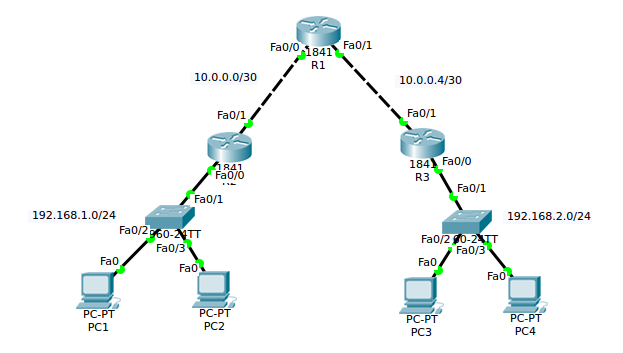
\includegraphics[width=0.6\textwidth]{1topo}
    \caption{Troubleshooting topology }
    \label{fig:1topo}
\end{figure}

\begin{itemize}
\item Hosts 
    \subitem Check if interfaces are \textit{up}.
    \subitem Check the IP address and subnet mask.
    \subitem Check the default gateway address.
\item Switches
    \subitem Check that the interfaces are up.
\item Routers
    \subitem The interfaces are \textit{up}.
    \subitem The IP address of the interfaces.
    \subitem The routing protocol RIPv2 is done correctly. That is they have the information about the networks that are connected. 
\item Cabling 
    \subitem All the cables are connected to correct interfaces with proper cables.
\end{itemize}


\subsection{Checking connectivity}

We check for connectivity between the nodes by running the \textbf{ping} command. As can be seen in Figure \ref{fig:1ping}. 

\begin{figure}
    \centering
    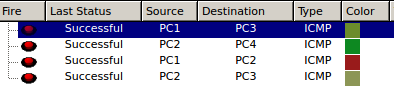
\includegraphics[width=0.6\textwidth]{1ping}
    \caption{Connectivity of the hosts in Topology \ref{fig:1topo}}
    \label{fig:1ping}
\end{figure}

\section{RIP routing table update}

\subsection{Downloading}

Download the 'RIP.pkt' file from Fronter and open it in PacketTracer.
The topology can be seen in Figure \ref{fig:2topo}.

\begin{figure}[h]
    \centering
    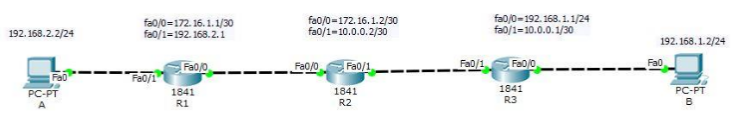
\includegraphics[width=\textwidth]{2topo}
    \caption{Topology for RIP.pkt}
    \label{fig:2topo}
\end{figure}

\subsection{Debuging RIP}

We use the \textbf{debug ip rip} command to see the RIP communications between the routers. 

\subsection{Inspecting RIP message}

Now we turn the interface fa0/0 off at R3 and inspect the RIP messages at R2. Router2 (R2) does not receive any update from Router3 (R3) on  Fa0/1, but it periodically recieves update from R1. 

\begin{verbatim}
\%LINEPROTO-5-UPDOWN: Line protocol on Interface FastEthernet0/1, changed state to down
RIP: received v2 update from 172.16.1.1 on FastEthernet0/0
      192.168.2.0/24 via 0.0.0.0 in 1 hops
RIP: sending  v2 update to 224.0.0.9 via FastEthernet0/0 (172.16.1.2)
RIP: build update entries
      192.168.1.0/24 via 0.0.0.0, metric 16, tag 0
RIP: received v2 update from 172.16.1.1 on FastEthernet0/0
      192.168.2.0/24 via 0.0.0.0 in 1 hops
\end{verbatim}

\subsection{RIP routing information distribution}

RIP updates the other routers only with the routes it knows. So if a link is down no update is sent.
We can check the routing table at R1 to see what happens. 
\begin{verbatim}
Router#show ip route
...
...
     10.0.0.0/30 is subnetted, 1 subnets
R       10.0.0.0 [120/1] via 172.16.1.2, 00:00:12, FastEthernet0/0
     172.16.0.0/30 is subnetted, 1 subnets
C       172.16.1.0 is directly connected, FastEthernet0/0
R    192.168.1.0/24 is possibly down, routing via 172.16.1.2, FastEthernet0/0
C    192.168.2.0/24 is directly connected, FastEthernet0/1
Router#

\end{verbatim}

First we see that R1 assumes that the 192.168.1.0/24 is possibly down but after fast forwarding the time it deletes the route to 192.168.1.0/24 as can be seen below,  when it does not get any more updates about the route to 192.168.1.0/24.

\begin{verbatim}
Router#show ip route
...
...
     10.0.0.0/30 is subnetted, 1 subnets
R       10.0.0.0 [120/1] via 172.16.1.2, 00:00:17, FastEthernet0/0
     172.16.0.0/30 is subnetted, 1 subnets
C       172.16.1.0 is directly connected, FastEthernet0/0
C    192.168.2.0/24 is directly connected, FastEthernet0/1
Router#
\end{verbatim}


\subsection{Administrative Distances and routing table}

We can see the routing table of R2 in Figure \ref{fig:2eR2route}. This shows which routing protocol it is using and gives a list of all the routing protocols and its 'short name'. 
\begin{figure}
    \centering
    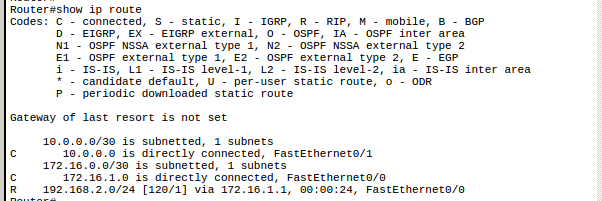
\includegraphics[width=\textwidth]{2eR2route}
    \caption{R2 routing table}
    \label{fig:2eR2route}
\end{figure}

The administrative distance for some of the different protocols can be seen in Table \ref{tab:2admindist}.

\begin{table}[h]
    \centering
    \begin{tabular}{|c|c|}
         \hline
         Routing Protocol & Administrative Distance \\
         \hline 
         Connected interface & 0 \\
         Static Route & 1 \\
         EIGRP & 5\\ 
         BGP & 20 \\
         OSPF & 110 \\
         RIP & 120 \\
         Unknown & 255 \\         
    \end{tabular}
    \caption{Administrative Distance of different routing protocols}
    \label{tab:2admindist}
\end{table}

\subsection{Multicast Address}
The purpose of the multicast address is to send the packets to multiple destinations, but not all, at the same time. The multicast address used by RIP to update the routing table is 224.0.0.9.
The different multicast addresses for the different protocols can be seen in Table \ref{tab:2muladd}. 
\begin{table}[h]
    \centering
    \begin{tabular}{|c|c|}
         \hline 
         Routing Protocol & Multicast Address  \\
         \hline 
         RIP & 224.0.0.9 \\
         OSPF & 224.0.0.5\\
         OSPF designated & 224.0.0.6\\
    \end{tabular}
    \caption{Multicast addresses of different Routing Protocols.}
    \label{tab:2muladd}
\end{table}

\section{OSPF routing table update}

\subsection{Downloading}
Downloading the 'OSPF.pkt' from fronter and opening it in PackerTracer. The network topology can be seen in Figure \ref{fig:3topo}


\begin{figure}[h]
    \centering
    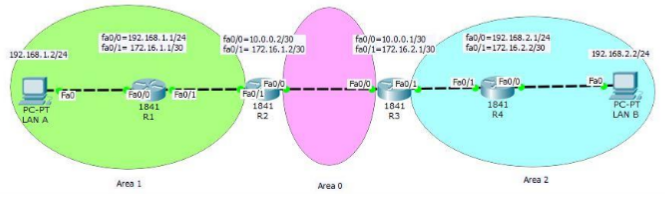
\includegraphics[width=\textwidth]{3topo}
    \caption{Topology for OSPF.pkt}
    \label{fig:3topo}
\end{figure}


\subsection{Checking connectivity}
First we check the connectivity from PC1 to PC2 with the \textbf{ping} command. There is  connectivity between the two hosts.

\subsection{Enabling debugging}

I use the command \textbf{debug ip routing} to enable debugging of ip routing, at R1.

\subsection{Inspecting communications}

I shutdown the interface fa0/0 at R4, and then inspect the messages at R1.
I get the following message at R1:

\begin{verbatim}
Router#RT: del 192.168.2.0 via 172.16.1.2, ospf metric [110/4]
RT: delete network route to 192.168.2.0
RT: NET-RED 192.168.2.0/24
\end{verbatim}

\subsubsection{Routing table update}

As we saw previously that R1 got updated if there was any changes to the network topology compared to RIP where it would periodically check for connectivity and assume that the router was down if it did not get any updates from it and then delete after a certain amount of time passes.  The DR and BDR does not change when the interface is down. This can be checked by running the \textbf{show ip ospf interface} command. 

Then we turn on the R4 interface fa0/0 by using the command \textbf{no shutdown}, in the interface. 
\begin{verbatim}
Router(config)#interface FastEthernet0/0
Router(config-if)#no shutdown
\end{verbatim}

\subsubsection{Standard area and Stub area}

First we check the routing table at R4 using the \textbf{show ip route} command. This can be seen in Figure \ref{fig:3froute1}.

\begin{figure}[h]
    \centering
    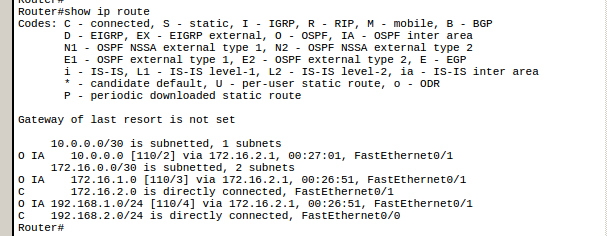
\includegraphics[width=0.7\textwidth]{3froute1}
    \caption{The routing table of R2}
    \label{fig:3froute1}
\end{figure}

Then we change the standard area, Area 2 to a stub area. We use the following commands to change the ospf area of a router from Standard to stub. 
\begin{verbatim}
Router#conf t
Router(config)#router ospf 1
Router(config-router)#area 2 stub
\end{verbatim}

\part{Configuring OSPF and BGP }

\subsection{Multi-area OSPF (PacketTracer)}

First we set the IP addresses with subnet masks at the host and then at the routers according to the configurations as seen in Figure \ref{fig:4topo}. We also set up the default gateway of the hosts to the router they are connected to.
\begin{figure}
    \centering
    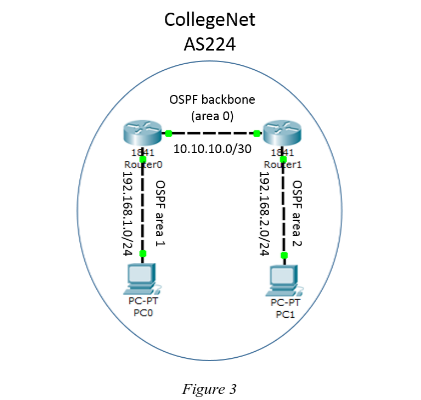
\includegraphics[width=0.7\textwidth]{4topo}
    \caption{Topology as shown in Figure 4 of Assignment 10.}
    \label{fig:4topo}
\end{figure}

Then we set up the OSPF routing protocol at the routers. We specify each interface to different areas. The commands used is seen below:
\begin{verbatim}
Router>enable 
Router#conf t
Enter configuration commands, one per line.  End with CNTL/Z.
Router(config)#router ospf 1
Router(config-router)#network 192.168.2.0 255.255.255.0 area 2
Router(config-router)#network 10.10.10.0 255.255.255.252 area 0 
\end{verbatim}

Then we check connectivity among the hosts, as seen in Figure \ref{fig:4ping} we have full connectivity. 

\begin{figure}
    \centering
    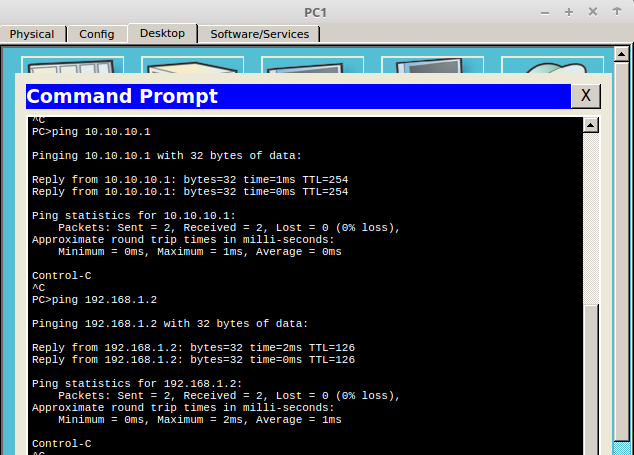
\includegraphics[width=0.6\textwidth]{4ping}
    \caption{Checking connectivity between hosts. Here we \textit{ping} Router0 and PC0 respectively from PC1. }
    \label{fig:4ping}
\end{figure}

\subsection{BGP with many ASes (PacketTracer)}

First we create the topology shown in Figure \ref{fig:5topo}. And assign the IP addresses to the hosts and the routers. We set the default gateways for the hosts. Then we configure the OSPF routing for Router 0-3. As done in the previous assignment. 

\begin{figure}[h]
    \centering
    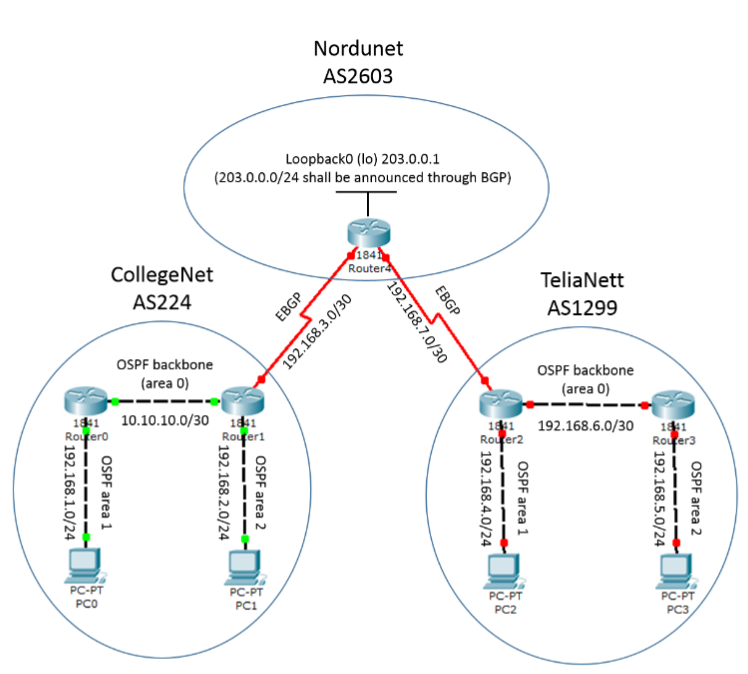
\includegraphics[width=\textwidth]{5topo}
    \caption{The topology for task}
    \label{fig:5topo}
\end{figure}


Then we configure Router4, Router3 and Router1. We add the \textit{BGP} routing protocol to the three routers with its corresponding AS-es. Then we add the neighboring \textit{bgp} router to its routing protocol using the \textbf{neighbor 192.168.7.1 remote-as 2603} command. All the neighbours with the BGP needs to be specified. Router4 has neighbor Router1 and Router2. Router1 has Router4 and Router2 has Router4 as well. After this is done we need to distribut the route to the other networks. This is done using the command \textbf{redistribute ospf 1} to redistribute the OSPF routes to the BGP router, and the command \textbf{redistribute bgp 1299} to redistribute the BGP routes to the OSPF routers. 

Then we check the connectivity, and as seen in Figure \ref{fig:5ping}.

\begin{figure}[h]
    \centering
    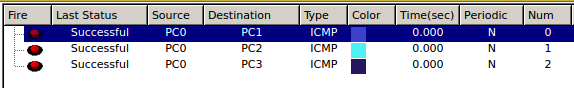
\includegraphics[width=\textwidth]{5ping}
    \caption{Checking connectivity between all the hosts.}
    \label{fig:5ping}
\end{figure}


\subsubsection{Router4 Configuration file}
\begin{verbatim}
    Building configuration...

Current configuration : 947 bytes
!
version 12.4
no service timestamps log datetime msec
no service timestamps debug datetime msec
no service password-encryption
!
hostname Router
!
no ip cef
no ipv6 cef
!
spanning-tree mode pvst
!
interface Loopback0
 ip address 203.0.0.1 255.255.255.0
!
interface FastEthernet0/0
 no ip address
 duplex auto
 speed auto
 shutdown
!
interface FastEthernet0/1
 no ip address
 duplex auto
 speed auto
 shutdown
!
interface Serial0/1/0
 ip address 192.168.3.1 255.255.255.252
 clock rate 2000000
!
interface Serial0/1/1
 ip address 192.168.7.1 255.255.255.252
 clock rate 2000000
!
interface Vlan1
 no ip address
 shutdown
!
router bgp 500
 bgp log-neighbor-changes
 no synchronization
 neighbor 192.168.7.2 remote-as 700
 neighbor 192.168.3.2 remote-as 600
 network 203.0.0.0
!
ip classless
!
ip flow-export version 9
!
no cdp run
!
line con 0
!
line aux 0
!
line vty 0 4
 login
!
end
\end{verbatim}


\subsubsection{Router1 Configuration}
\begin{verbatim}
    Current configuration : 957 bytes
!
version 12.4
no service timestamps log datetime msec
no service timestamps debug datetime msec
no service password-encryption
!
hostname Router
!
ip cef
no ipv6 cef
!
spanning-tree mode pvst
!
interface FastEthernet0/0
 ip address 10.10.10.2 255.255.255.252
 duplex auto
 speed auto
!
interface FastEthernet0/1
 ip address 192.168.2.1 255.255.255.0
 duplex auto
 speed auto
!
interface Serial0/1/0
 ip address 192.168.3.2 255.255.255.252
!
interface Serial0/1/1
 no ip address
 clock rate 2000000
!
interface Vlan1
 no ip address
 shutdown
!
router ospf 1
 log-adjacency-changes
 redistribute bgp 600 
 network 192.168.2.0 0.0.0.255 area 2
 network 10.10.10.0 0.0.0.3 area 0
!
router bgp 600
 bgp log-neighbor-changes
 no synchronization
 neighbor 192.168.3.1 remote-as 500
 redistribute ospf 1 
!
ip classless
!
ip flow-export version 9
!
line con 0
!
line aux 0
!
line vty 0 4
 login
!
end
\end{verbatim}

\subsubsection{Router2 Configuration file}
\begin{verbatim}

Current configuration : 959 bytes
!
version 12.4
no service timestamps log datetime msec
no service timestamps debug datetime msec
no service password-encryption
!
hostname Router
!
ip cef
no ipv6 cef
!
spanning-tree mode pvst
!
interface FastEthernet0/0
 ip address 192.168.6.1 255.255.255.252
 duplex auto
 speed auto
!
interface FastEthernet0/1
 ip address 192.168.4.1 255.255.255.0
 duplex auto
 speed auto
!
interface Serial0/1/0
 ip address 192.168.7.2 255.255.255.252
!
interface Serial0/1/1
 no ip address
 clock rate 2000000
!
interface Vlan1
 no ip address
 shutdown
!
router ospf 1
 log-adjacency-changes
 redistribute bgp 700 
 network 192.168.4.0 0.0.0.255 area 1
 network 192.168.6.0 0.0.0.3 area 0
!
router bgp 700
 bgp log-neighbor-changes
 no synchronization
 neighbor 192.168.7.1 remote-as 500
 redistribute ospf 1 
!
ip classless
!
ip flow-export version 9
!
line con 0
!
line aux 0
!
line vty 0 4
 login
!
end
\end{verbatim}

\end{document}
